\documentclass{acm_proc_article-sp}

\usepackage{graphicx}% Include figure files
\usepackage{caption}
\usepackage{subcaption}
\usepackage{dcolumn}% Align table columns on decimal point
\usepackage{bm}% bold math
\usepackage{amsmath}
\usepackage{float}
\usepackage{array}
\usepackage{verbatim}
\usepackage{tikz}
\usepackage{hyperref}% add hypertext capabilities
\usepackage{xcolor}
%\usepackage[mathlines]{lineno}% Enable numbering of text and display math
%\linenumbers\relax % Commence numbering lines


\usepackage{listings}
%\usepackage{footnote}
%\makesavenoteenv{table}
%\makesavenoteenv{table*}
%\makesavenoteenv{tabular}

\begin{document}

\title{Self-Organizing systems WS14\\
       Hexagonal SOM extension}

\numberofauthors{2}
\author{
Richard Plangger\\
\email{e1025637@student.tuwien.ac.at}
\alignauthor
Rene Koller\\
\email{eXXXXXXX@student.tuwien.ac.at}
\alignauthor
}

\date{\today}

\maketitle

\begin{abstract}
    This document describes our solution to the assignment
    to extend the SOM Toolbox to train and display a hexagonal
    SOM
\end{abstract}

\keywords{Self organizing systems, SOM, hexagonal, training}

\section{SOM Toolbox}

For this assignment we used the SOM Toolbox~\cite{somtoolbox}. Our solution
is based on the source code found in the section ``Download Latest'' and is
identified by the version ``0.7.5-4.svn4332''.

\section{Terminology}

As shown in Figure~\ref{fig:coord} both hexagonal and rectangular
use the same coordinate system to reference nodes from their memory.
There was no need to modify the array cell layout, but only adjust the
calculation for the grid neighbors. The major
difference while using hexagonal grid system is that there are not only
four direct neighbors but six.

The neighbors using $(X/Y)$ as coordinate indices of $(1/1)$ in Figure~\ref{fig:coord-rect}
are $\{(1/2),(2/1),(1/0),(0/1)\}$. In Figure~\ref{fig:coord-hex} they are $\{(1/2),(2/2),(2/1),(2/0),(1/0),(0/1)\}$.

The hexagonal grid is rendered ``pointy top''\footnote{The hexagon is rotated in such a way that an edge points up} and every second row is shifted half width of a
cell to the left.

\begin{figure}
    \begin{subfigure}{1\linewidth}
    \centering
    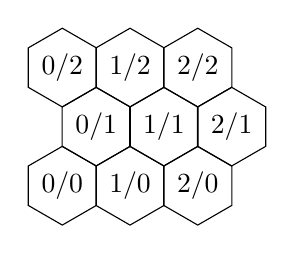
\begin{tikzpicture}
        \foreach \off / \x / \y in {0/0/0,0/1/0,0/2/0,0.43cm/0/1,0.43cm/1/1,0.43cm/2/1,0/0/2,0/1/2,0/2/2} {
            \draw ({\off + \x*0.86cm},{0.75cm * \y}) -- ++(30:0.5cm)
              \foreach \r in {90,150,210,270,330} { -- ++(\r:0.5cm) }
              -- cycle;
          \draw ({\off + \x*0.86cm},{0.75cm * \y + 0.5cm}) node {\x/\y};
        };
    \end{tikzpicture}
    \caption{hexagonal}
    \label{fig:coord-hex}
    \end{subfigure}

    \begin{subfigure}{1\linewidth}
        \centering
    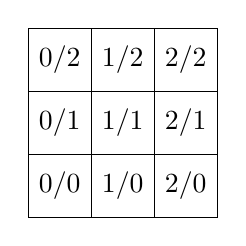
\begin{tikzpicture}
        \foreach \off / \x / \y in {0/0/0,0/1/0,0/2/0,0.43cm/0/1,0.43cm/1/1,0.43cm/2/1,0/0/2,0/1/2,0/2/2} {
            \draw ({0.8cm * \x},{0.8cm * \y})
              -- ++({0.8cm},{0})
              -- ++({0},{0.8cm})
              -- ++({-0.8cm},{0})
              -- cycle;
          \draw ({\x*0.8cm + 0.4cm},{0.8cm * \y + 0.4cm}) node {\x/\y};
        };
    \end{tikzpicture}
    \caption{rectangular}
    \label{fig:coord-rect}
    \end{subfigure}
    \caption{Coordinate system and layout}
    \label{fig:coord}
\end{figure}

To abstract the grid neighborhood, geometric layout and rendering from the actual 3d \lstinline!Unit! array
representation a new interface has been introduced. The interface \lstinline!GridGeometry! is the base abstraction
to be able to calculate shapes, center of the shapes and the grid neighbors.

\section{Hexagonal Training}

By examining the training process implemented in \lstinline!GrowingLayer! we have identified the following two strategies.
First there is the single threaded training calculating the neighborhood using the function presented in the lecture:
\[
    h_{ci} = \alpha \times exp(-\frac{dist(winner,unit)^2}{2\sigma^2})
\]
In the function \lstinline!updateUnitsInArea! $h_{ci}$ is the used to updated the weight vectors for each unit.

The second strategy is called batch SOM that, similar to the first strategy, uses the squared distance to the neighbors
to mark the activation. It then updates the weight vector of every node by assigning the mean value of all mapped input
data samples in the neighborhood.

Since the algorithms are so similar we decided not to duplicate the SOM training code contained in \lstinline!GrowingLayer! but
rather just abstract the distance measures. The main advantage of our approach is that all features of the growing layer (such as adding and removing columns for a non static SOM) can now also be used with a hexagonal grid.

Both strategies mentioned earlier solely rely on the distance measure in the grid geometry.
Figure~\ref{fig:hci-coord-rect} illustrates the rectangular distance measurement.
The inner dashed circle has an euclidean distance of $\sqrt{1} = 1$ to
the unit center at position $(1,1)$. The geometry layout in the code does not calculate the distance from the center of
the unit square, but from the corner (lower left). The distance for the second dashed circle has an euclidean distance of $\sqrt{2} \approx 1.14$ and finally the last circle has a distance from the unit (1/1) of $\sqrt{4} = 2$.

To achieve the same distances in a hexagonal grid our approach is visualized in Figure~\ref{fig:hci-coord-hex}.
The inner circle has a distance of $1$ to all of his 6 neighbors. To achieve this distance metric 
we use the rectangular unit space which with an unit $u$ from any neighboring unit. The hexagon grid forces deformation
of the shapes the following formulas are used to calculate the grid.

\begin{itemize}
    \item Hexagonal width using a reference unit $u$ (e.g cm) is $1$. Trivially
        $ h_w(u) = u; h_w(1) = 1 $
    \item Hexagonal height using a reference unit $u$ \\
        $ h_h(u) = u \times \frac{2}{\sqrt{3}} * \frac{3}{4}; h_h(1) \approx 0.86 $
    \item Hexagonal shift\footnote{Note that the hexagonal shift only returns a non zero
    	value for every second row.} using a reference unit $u$ \\
        \[ h_s(u) = \left\{
               \begin{array} {l l}
                   h_w(u)/2 & \mathrm{if}\ index(row)\mod 2 = 1 \\
                   0 & \mathrm{otherwise}
               \end{array}
               \right.\]
        
    \item Euclidean distance formula. 
    \begin{align*}
        d(p_1,p_2) & = \sqrt{ A^2 + B^2 }\\
        A & = (h_w(1) * p_2.x + h_s(1)) \\
          &- (h_w(1) * p_1.x + h_s(1))\\
        B & = (h_h(1) * p_2.y) - (h_h(1) * p_1.y)
    \end{align*}
    $p_x$ is a point in the rectangular grid. The dot-operator $x$ and $y$
    (e.g. $p_1.x$) get the rectangular position. Thus $d(p_1,p_2)$ is just the
    euclidean distance adjusted by the hexagonal shape width and height
    and every second row shifted by half of the width.
\end{itemize}

\begin{table}
	\centering
	\begin{tabular}{|l|c|c|c|c|}
		\hline
		  & $r=1$& $r=2$ & $r=3$ & $r=4$ \\
		\hline
		Rect. $\mathrm{euclidean}^2$ & 4 & 8 & 8 & 12 \\
		\hline
		Hex. $\mathrm{euclidean}^2$ & 6 & 6 & 12 & 18 \\
		\hline
		\hline
		Rect. $\mathrm{euclidean}$ & 4 & 12 &  28 & 48 \\
		\hline
		Hex. $\mathrm{euclidean}$ & 6 & 18 & 36 & 60 \\
		\hline
	\end{tabular}
	\caption{Neighbouring units using different grid layout and distance measures. Columns show different radius values $r$.}
	\label{tab:neighbours} 
\end{table}

Table~\ref{tab:neighbours} shows the amount of neighbors in a $100\times100$ grid. The unit to measure the distance from is located at index $(50,50)$. Notably using the squared euclidean distance it can happen that for a radius of 2 hexagonal grid has less neighbors than the rectangular one. This can also be observed in Figure~\ref{fig:hci-coord-hex} at position $(0,0)$. The squared distance from $(1,1)$ is 3 which is greater than 2. The black solid circle shows a radius of distance 2.
For all others we have observed and for the subset we added to the table hexagonal has always more neighbors than the rectangular one.

Figure~\ref{fig:hci-coord-hex} and~\ref{fig:hci-coord-rect} show the activation of neighbors using three dashed circles. Each circle intersects exactly with 6 nodes centers in the hexagonal grid and 4 nodes in the rectangular grid.

\colorlet{c1}{red}
\colorlet{c2}{violet}
\colorlet{c3}{cyan}
\colorlet{c4}{black}

\begin{figure}
    \begin{subfigure}{1\linewidth}
    \centering
    \begin{tikzpicture}
        \foreach \off / \x / \y in {0/0/0,0/1/0,0/2/0,0/3/0,
                         0.43cm/0/1,0.43cm/1/1,0.43cm/2/1,0.43cm/3/1,
                         0/0/2,0/1/2,0/2/2,0/3/2,
                         0.43cm/0/3,0.43cm/1/3,0.43cm/2/3,0.43cm/3/3} {
            \draw ({\off + \x*0.86cm},{0.75cm * \y}) -- ++(30:0.5cm)
              \foreach \r in {90,150,210,270,330} { -- ++(\r:0.5cm) }
              -- cycle;
          \draw ({\off + \x*0.86cm},{0.75cm * \y + 0.5cm}) node {\x/\y};
        };

        \draw [fill,black] ({0.86cm * 1 + 0.43cm},{0.75cm * 1 + 0.5cm}) circle [radius=0.06cm];

        \draw [dashed,c1] ({0.86cm * 1 + 0.43cm},{0.75cm * 1 + 0.5cm}) circle [radius=0.86cm];
        \draw [dashed,c2] ({0.86cm * 1 + 0.43cm},{0.75cm * 1 + 0.5cm}) circle [radius={0.75cm * 2}];
        \draw [dashed,c3] ({0.86cm * 1 + 0.43cm},{0.75cm * 1 + 0.5cm}) circle [radius={2.2821cm}];
        \draw [c4] ({0.86cm * 1 + 0.43cm},{0.75cm * 1 + 0.5cm}) circle [radius={0.86cm * 2}];
        \foreach \off / \x / \y in {0/1/0,0/2/0,0.43cm/0/1,0.43cm/2/1,0/1/2,0/2/2} {
            \draw [fill,c1] ({\off + 0.86cm * \x},{0.75cm * \y + 0.5cm}) circle [radius=0.06cm];
        };
        \foreach \off / \x / \y in {0/0/0,0/0/2,0/3/2,0/3/0,0.43cm/1/3} {
            \draw [fill, c2] ({\off + 0.86cm * \x},{0.75cm * \y + 0.5cm}) circle [radius=0.06cm];
        };
        \draw [fill,c3] ({0.43cm + 0.86cm * 3},{0.75cm * 3 + 0.5cm}) circle [radius=0.06cm];
    \end{tikzpicture}
    \caption{hexagonal}
    \label{fig:hci-coord-hex}
    \end{subfigure}

    \begin{subfigure}{1\linewidth}
        \centering
    \begin{tikzpicture}
        \foreach \off / \x / \y in {0/0/0,0/1/0,0/2/0,0.43cm/0/1,0.43cm/1/1,0.43cm/2/1,0/0/2,0/1/2,0/2/2} {
            \draw ({0.8cm * \x},{0.8cm * \y})
              -- ++({0.8cm},{0})
              -- ++({0},{0.8cm})
              -- ++({-0.8cm},{0})
              -- cycle;
          \draw ({\x*0.8cm + 0.4cm},{0.8cm * \y + 0.4cm}) node {\x/\y};
        };

        \draw [dashed,c1] ({0.8cm * 1},{0.8cm * 1}) circle [radius=0.8cm];
        \draw [fill,c1] ({0.8cm * 1},{0.8cm * 0}) circle [radius=0.06cm];
        \draw [fill,c1] ({0.8cm * 0},{0.8cm * 1}) circle [radius=0.06cm];
        \draw [fill,c1] ({0.8cm * 2},{0.8cm * 1}) circle [radius=0.06cm];
        \draw [fill,c1] ({0.8cm * 1},{0.8cm * 2}) circle [radius=0.06cm];

        \draw [fill,black] ({0.8cm * 1},{0.8cm * 1}) circle [radius=0.06cm];

        \draw [dashed,c2] ({0.8cm * 1},{0.8cm * 1}) circle [radius={1.1313cm}];
        \foreach \x / \y in {0/0,2/0,2/2,0/2} {
            \draw [fill,c2] ({0.8cm * \x},{0.8cm * \y}) circle [radius=0.06cm];
        }

        \draw [dashed,c3] ({0.8cm * 1},{0.8cm * 1}) circle [radius={0.8cm * 2}];
        \foreach \x / \y in {3/1,1/3} {
            \draw [fill,c3] ({0.8cm * \x},{0.8cm * \y}) circle [radius=0.06cm];
        }
    \end{tikzpicture}
    \caption{rectangular}
    \label{fig:hci-coord-rect}
    \end{subfigure}
    \caption{Coordinate system and layout}
    \label{fig:coord}
\end{figure}

\section{Visualisation}

We have picked two data sets that we will compare in the Sections~\ref{sec:iris} and~\ref{sec:chain-link}. In the following we compiled a list of visualizations that we modified to work for both grid systems.

\begin{itemize}
	\item Activity Histogram
	\item Hit Histogram
	\item U-Matrix
	\item D-Matrix
	\item P-Matrix
	\item Fuzzy Colouring
	\item Neighbourhood Graph radius
	\item Neighbourhood Graph KNN (K-nearest neighbour)
	
	\item Quantization Error
	\item Mean Quantization Error
	\item Topographic Error (4/8 units)
\end{itemize}

In every Figure we show the rectangular SOM on the left and the hexagonal on the right hand side.

\newcommand{\cmprecthex}[5]
{
	\begin{figure}
		\begin{subfigure}{0.49\linewidth}
			\includegraphics*[width=\linewidth]{img/#1-#2}
			\caption{#5}
			\label{fig:#1-#2-rect}
		\end{subfigure}
		\begin{subfigure}{0.49\linewidth}
			\includegraphics[width=\linewidth]{img/#1-#2-hex}
			\caption{#4}
			\label{fig:#1-#2-hex}
		\end{subfigure}
		\caption{#3}
		\label{fig:#1-#2}
	\end{figure}
}


\subsection{Iris}
\label{sec:iris}

\subsection{Chain Link}
\label{sec:chain-link}

\cmprecthex{cl}{activity}{Activity histogram. Default referent unit}{Hexagonal}{Rectangular}
\cmprecthex{cl}{dmatrix}{D-Matrix}{Hexagonal}{Rectangular}
\cmprecthex{cl}{pmatrix}{P-Matrix}{Hexagonal}{Rectangular}
\cmprecthex{cl}{umatrix}{U-Matrix}{Hexagonal}{Rectangular}
\cmprecthex{cl}{dist}{Distortion}{Hexagonal}{Rectangular}
\cmprecthex{cl}{qe}{QE}{Hexagonal}{Rectangular}
\cmprecthex{cl}{mqe}{MQE}{Hexagonal}{Rectangular}
\cmprecthex{cl}{mqe}{Topo 4}{Hexagonal}{Rectangular}
\cmprecthex{cl}{fuzzy-colouring}{Fuzzy coloring}{Hexagonal}{Rectangular}
\cmprecthex{cl}{nh-knn-1}{Neighbourhood KNN 1}{Hexagonal}{Rectangular}
\cmprecthex{cl}{nh-knn-2}{Neighbourhood KNN 2}{Hexagonal}{Rectangular}
\cmprecthex{cl}{nh-knn-3}{Neighbourhood KNN 3}{Hexagonal}{Rectangular}
\cmprecthex{cl}{nh-radius-0,1}{Neighbourhood Graph Radius 0.1}{Hexagonal}{Rectangular}
\cmprecthex{cl}{nh-radius-0,2}{Neighbourhood Graph Radius 0.2}{Hexagonal}{Rectangular}
\cmprecthex{cl}{nh-radius-0,3}{Neighbourhood Graph Radius 0.3}{Hexagonal}{Rectangular}



\bibliography{ref}
\bibliographystyle{plain}

\end{document}
